% !TEX root = ./main.tex

\chapter{Internship company} % (fold)
\label{sec:voorstelling}

I did my internship at Showpad in Ghent. Showpad is a software as a service start-up that was founded in 2011 by ex-employees of In The Pocket, a mobile agency. Since then the company has grown at a fast pace, today Showpad has over 1000 customers and over 200 employees in offices in Ghent, London, San Francisco and Portland \cite{showpad-grow}.

Showpad provides a B2B service that aims to align marketing and sales departments by making marketing materials easily accessible and shareable. Showpad achieves this by hosting a platform and developing native applications for Android and iOS as well as a web application.

Showpad aims its service at enterprise customers with over 250 employees. Showpad's customers include Coca-cola, Audi, Johnson \& Johnson and many other big names \cite{showpad}. These customers pay Showpad a monthly subscription fee per user for the SaaS.

Showpad has been doubling it's revenue every year for the past 4 years. At the end of 2015 Showpad's annual recurring revenue exceeded \$10 million \cite{showpad-arr}. In May 2016 Showpad closed a \$50 million funding round led by Insight Venture Partners \cite{showpad-grow}.

\section{Internal structure}

Internally Showpad is divided into 5 departments, listed in order of descending size these are: customer success, engineering, sales, marketing and employee success. As can be deduced from this order, Showpad invests heavily in customer experience. Showpad prides itself on its very short customer issue cycle time and a strong synergy between customer success and engineering is essential to achieve this.

\subsection{Engineering}

\subsubsection{Teams}

The engineering department is divided into 6 smaller teams with around 10 members. These teams are not divided by product or discipline but rather by the functionality they implement and maintain. An example of this is the create \& present team. That team maintains all user functionality related to creating and presenting content in Showpad.

The engineering teams in Showpad are discover \& measure, distribute \& collaborate, share \& personalize and create \& present. Every team consists of front-end and back-end developers as well at least one quality assurance engineer and a team coach. There are also two teams that aren't linked to specific functionality. Those teams are the mobile \& learn team and the architecture team because these are two smaller teams that can't be linked to a specific user functionality. Even though these are separate teams there is still a lot of collaboration between different teams.

During my internship I was a part of the share \& personalize team. This team maintains all features related to sharing and personalizing content in all Showpad products (except the mobile apps).


\subsubsection{Guilds}

In Showpad engineering there are guilds for every development discipline. These 4 guilds are the front-end guild, the back-end guild, the architecture guild and the QA guild. Every guild has a separate group chat to share interesting articles or new developments in their areas of expertise. The guilds also have a weekly meeting to talk about any topic within their field. In these meetings every guild member has the opportunity to give a presentation or workshop on something they find interesting in their discipline.

During my internship I was a part of the front-end guild. The last week of my internship I gave a presentation during the guild. The presentation was about common pitfalls in functional reactive programming and included small code recipes and demos \cite{slides}.

\subsubsection{Kanban}

Every team has a Kanban board \cite{kanban} on which they receive and create new development tickets. These tickets are then taken through a development cycle which includes a peer code review and a testing session (see figure~\ref{figure:flow}). Sometimes there are separate Kanban boards for epics. Epics are large features that typically require a long time in development and are not specific to one team. An example of an epic I took part in during my internship is the complete rewrite of the web application in Angular 2.

For distributing tickets between developers Showpad engineering uses a pull system instead of a push system. This means that developers self-assign tasks they feel comfortable working on instead of tasks being pushed to developers by a team coach.

\begin{figure}[H]
	\centering
	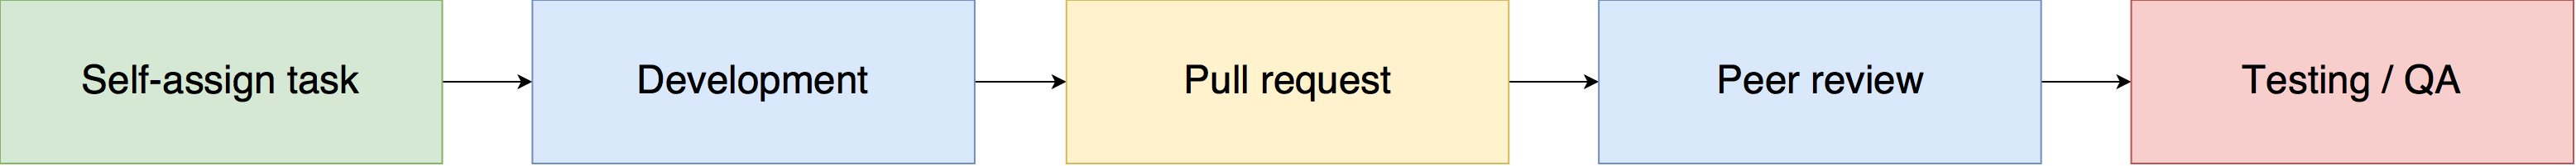
\includegraphics[width=1\textwidth]{flow}
	\caption{Ticket development cycle in Showpad}
	\label{figure:flow}
\end{figure}

\subsubsection{Continuous integration}

Showpad engineering puts a lot of effort into continuous integration and deployment. The development process is largely automated (see figure~\ref{figure:workflow}). Every commit that is pushed to a git repository gets built and tested automatically by a build server. Furthermore every pull request that is approved in a code review gets deployed to a minion where it gets tested by a QA engineer. If the QA engineer approves the changes and verifies the functionality the pull request will be deployed on the staging servers. On the staging servers a last sanity check is done to ensure everything is working. If there are no issues on staging the code will be added to a release and deployed to production in cycles of about a week on average. This very fast development cycle results in a rapidly improving product and a very quick response time to customer reported issues.

\begin{figure}[H]
	\centering
	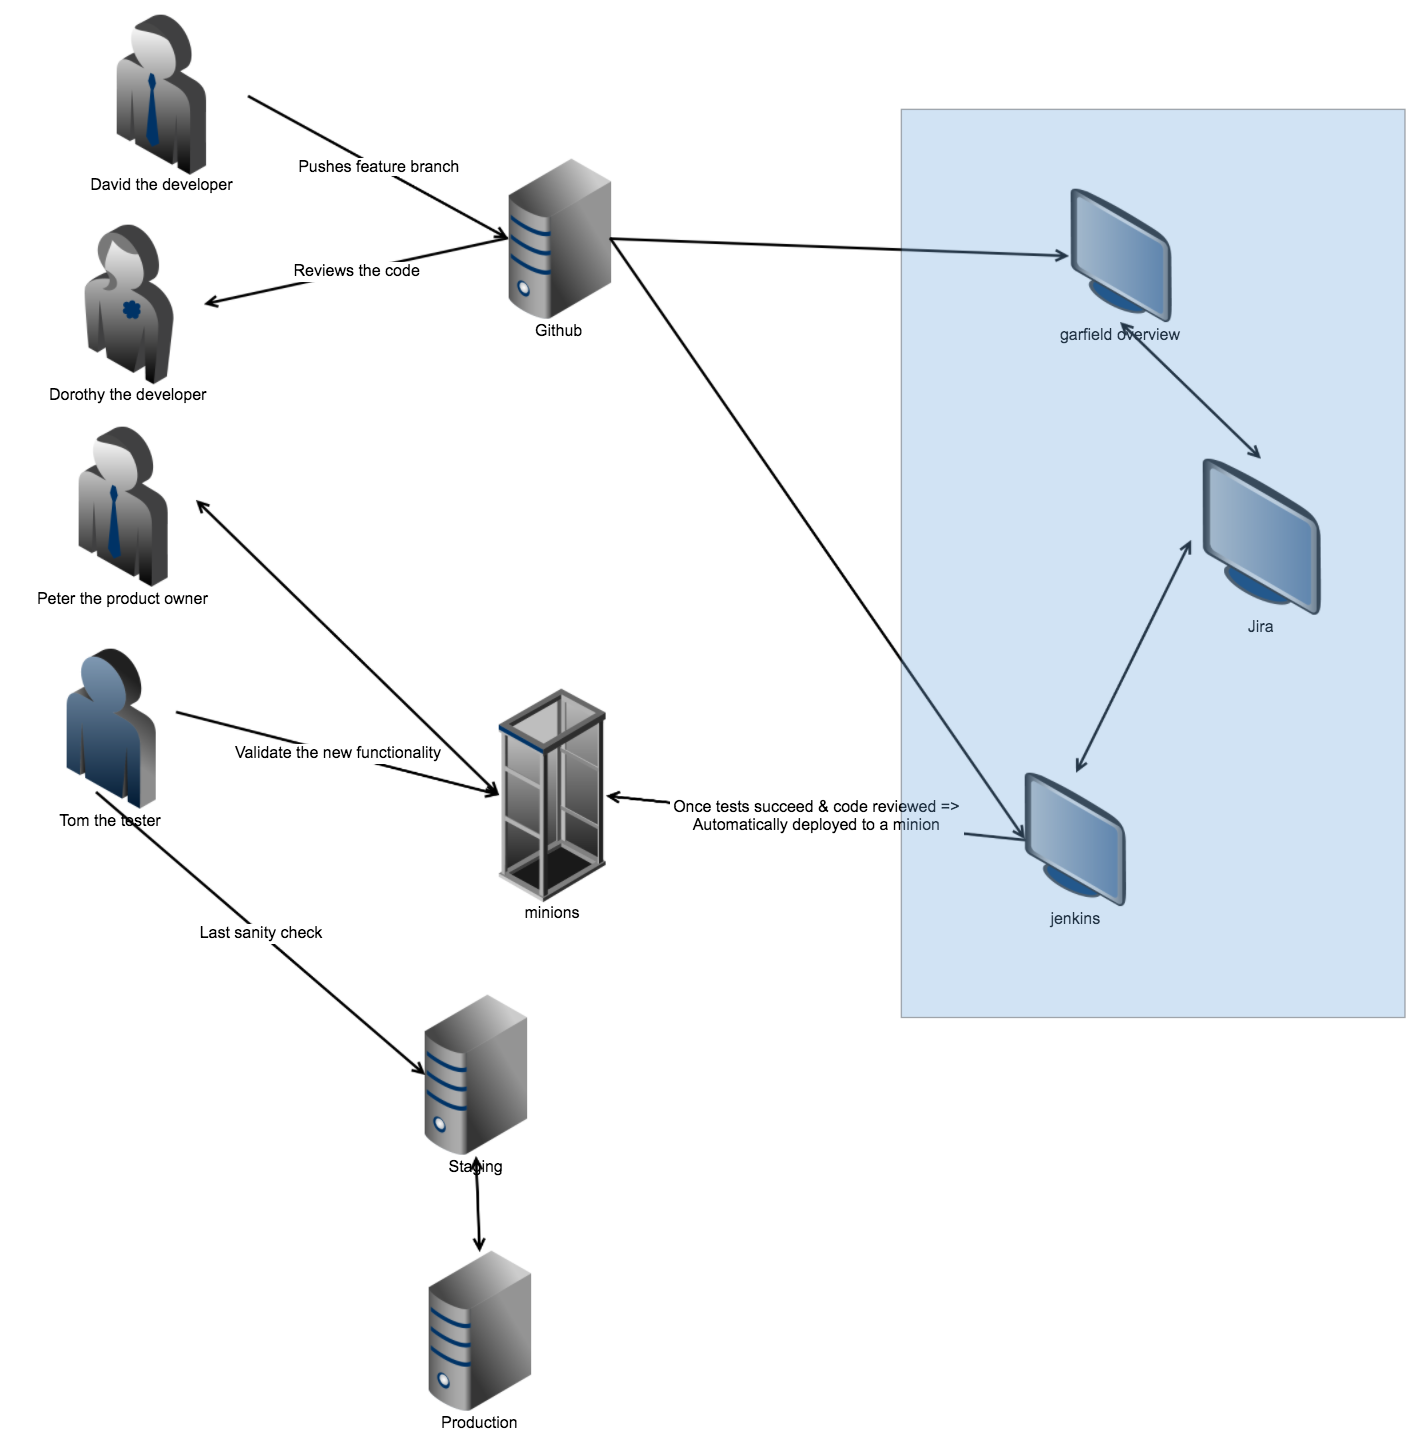
\includegraphics[width=1\textwidth]{integration}
	\caption{Showpad developer workflow diagram}
	\label{figure:workflow}
\end{figure}

\section{Culture}

Showpad has a very open culture that is typical for a start-up in the technology scene. The office is designed to be as open as possible to encourage interdepartmental collaboration and create a good atmosphere in general (see figure~\ref{figure:office}).

\begin{figure}[H]
	\centering
	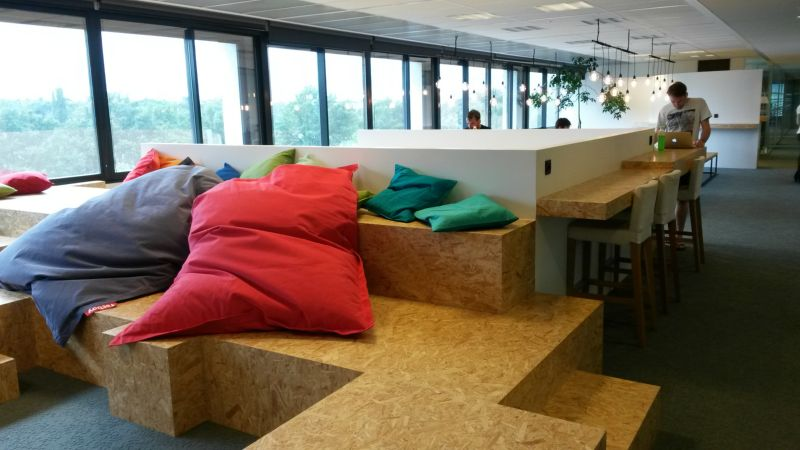
\includegraphics[width=0.9\textwidth]{office}
	\caption{Showpad office atmosphere}
	\label{figure:office}
\end{figure}

\subsection{Showings}

Showpad outlines 6 characteristics called showings that a good Showpad employee should have. These showings are shown in figure~\ref{figure:showings}.

\begin{figure}[H]
	\centering
	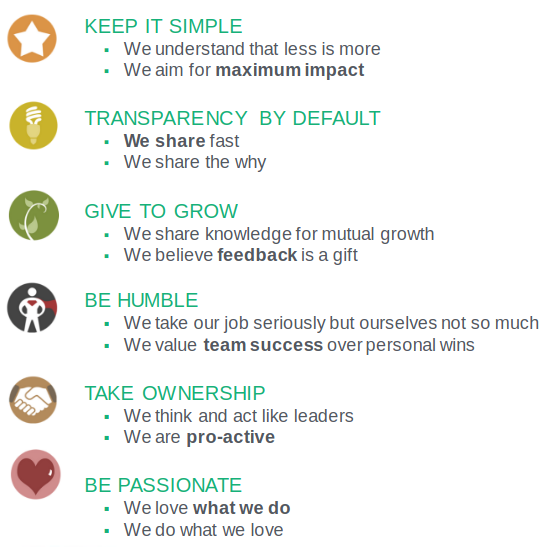
\includegraphics[width=0.6\textwidth]{showings}
	\caption{The 6 showings}
	\label{figure:showings}
\end{figure}

\subsection{Events}

Showpad organizes a lot of events for its employees and customers. Every Friday evening there is an event for all employees where they can have drinks together to set off the weekend. Every other week there is also a Showpie on Friday. This is an event where all employees in all offices get together in a video call and there is a moment to ask questions to the leadership. Sometimes Showpie also includes a speech or presentation by the CEO.

Showpad engineering organizes their own yearly developer conference in Ghent called GEARS \cite{showpad-gears}. This is a free event open to all web developers. The event hosts talks and presentations by Showpad engineers and external speakers from leading technology companies. There are open donations on the event that go to a charity of Showpad's choosing.

Lastly Showpad organizes a yearly event for its customers called Showtime. Showtime gives Showpad customers a chance to share their experience with the product \cite{showpad-showtime}.




